\documentclass{article}
\usepackage{malmacros}
\begin{document}

\section{Generalization Error}

In this section, the generalization error will be explored. The under-fitting and over-fitting zones are explained, and terms such as capacity, optimal capacity and generalization gap.

\subsection{Qa On Generalization Error}

\begin{figure}[H]
  \centering
    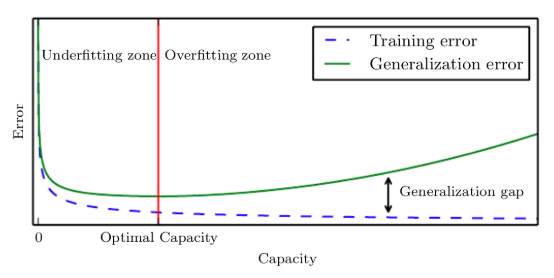
\includegraphics[width=0.9\textwidth]{error-vs-capacity}
    \caption{Error rate vs. Model capacity}
    \label{fig:Err_vs_cap}
\end{figure}

The generalization error is as described in the book on p. 29: The error rate of new cases, 
it is also known as the "out-of-sample error". And by evaluation and cross-validation on the test-set,
an estimation of this error rate can be found, which in turn tells you how well a model performs.
\\ \\
The "generalization error" can tell us wherther a model is over-fitting or under-fitting.
If the error rate of the training model is low, (i.e. Few mistakes are made under the training of the model),
but the "generalization error" is high (the error rate is high when the model is used on the test set),
then the model is "over-fitting". If in turn the error rate is high on both training and test set,
the model is "under-fitting".
\\ \\
In the figure above the curves depict the performance rate of the model, on both the training set and the validation set.
The graph is then separated into an under-fitting zone, and an over-fitting zone, which is divide the optimal capacity.
The capacity of a model is affected by things like the number of parameters used, (higher polynomial  means more parameters),
and how long the model is trained for (more iterations = longer training).
\\ \\
An example of under-fitting, is trying to fit a linear model, on a polynomial data set, the low capacity of the linear model,
leads to a bad fit, on both the training set, and validation set. It gives us low variance but a high bias. To combat this we could use a higher degree polynomial and by that increase the model capacity. This would create a better fit on training data, and lower the bias,
but the increased variance could mean that in generalizes more poorly. Which in turn could increase the gap between the training error and the generalization error, this is what is know as the "Generalization gap", which is usually the sign of over-fitting.
\\ \\
Optimal capacity is when the generalization error is at is minimum. A good way to reach optimal capacity is by using  "Early stopping".
This is when the model capacity is increased by running the model training for longer (more iterations), and then monitoring the generalization error. At a point it will reach a minimum and then start to increase again (going in to over-fitting). Early stopping is rolling back to stop at the point where the generalization error reached a global minimum.



\subsection{Qb A MSE-Epoch/Error Plot}

\begin{pyminted}
%matplotlib inline
import matplotlib
import matplotlib.pyplot as plt
import numpy as np

from sklearn.preprocessing import PolynomialFeatures, StandardScaler
from sklearn.pipeline import Pipeline
from sklearn.linear_model import SGDRegressor
from sklearn.model_selection import train_test_split
from sklearn.metrics import mean_squared_error

np.random.seed(42)

def GenerateData():
    m = 100
    X = 6 * np.random.rand(m, 1) - 3
    y = 2 + X + 0.5 * X**2 + np.random.randn(m, 1)
    return X, y

X, y = GenerateData()
X_train, X_val, y_train, y_val = train_test_split(X[:50], y[:50].ravel(), test_size=0.5, random_state=10)

poly_scaler = Pipeline([
        ("poly_features", PolynomialFeatures(degree=90, include_bias=False)),
        ("std_scaler", StandardScaler()),
    ])

X_train_poly_scaled = poly_scaler.fit_transform(X_train)
X_val_poly_scaled   = poly_scaler.transform(X_val)
\end{pyminted}

An \textbf{epoch} is each round the entire dataset is iterated over. It is needed when iterating through the full dataset several times. The reason for this can be to avoid underfitting. In the Train method in the code snippet below the epoch is the outer loop. In each epoch the same training values will be reused. During the an epoch \texttt{mse\_train} and \texttt{mse\_val} will be appended as \texttt{train\_errors} and \texttt{val\_errors}. In the end of the function after all epochs have been iterated through these are returned.

\begin{pyminted}
def Train(X_train, y_train, X_val, y_val, n_epochs, verbose=False):
    print("Training...n_epochs=",n_epochs)
    train_errors, val_errors = [], []
    
    sgd_reg = SGDRegressor(max_iter=1,
                           penalty=None,
                           eta0=0.0005,
                           warm_start=True,
                           learning_rate="constant",
                           tol=-float("inf"),
                           random_state=42)

    for epoch in range(n_epochs):
        sgd_reg.fit(X_train, y_train)
        y_train_predict = sgd_reg.predict(X_train)
        y_val_predict   = sgd_reg.predict(X_val)

        mse_train=mean_squared_error(y_train, y_train_predict)
        mse_val  =mean_squared_error(y_val  , y_val_predict)

        train_errors.append(mse_train)
        val_errors  .append(mse_val)
        if verbose:
            print(f"  epoch={epoch:4d}, mse_train={mse_train:4.2f}, mse_val={mse_val:4.2f}")

    return train_errors, val_errors

n_epochs = 500
train_errors, val_errors = Train(X_train_poly_scaled, y_train, X_val_poly_scaled, y_val, n_epochs, True)

best_epoch = np.argmin(val_errors)
best_val_rmse = np.sqrt(val_errors[best_epoch])

plt.figure(figsize=(7,4))
plt.annotate('Best model',
             xy=(best_epoch, best_val_rmse),
             xytext=(best_epoch, best_val_rmse + 1),
             ha="center",
             arrowprops=dict(facecolor='black', shrink=0.05),
             fontsize=16,
            )

best_val_rmse -= 0.03  # just to make the graph look better
plt.plot([0, n_epochs], [best_val_rmse, best_val_rmse], "k:", linewidth=2)
plt.plot(np.sqrt(val_errors), "r-", linewidth=3, label="Validation set")
plt.plot(np.sqrt(train_errors), "b--", linewidth=2, label="Training set")
plt.legend(loc="upper right", fontsize=14)
plt.xlabel("Epoch", fontsize=14)
plt.ylabel("RMSE", fontsize=14)
plt.show()
\end{pyminted}
\begin{pyconsole}
Training...n_epochs= 500
  epoch=   0, mse_train=11.85, mse_val=14.58
  epoch=   1, mse_train=11.51, mse_val=14.10
  epoch=   2, mse_train=11.15, mse_val=13.60
  epoch=   3, mse_train=10.81, mse_val=13.13
  epoch=   4, mse_train=10.49, mse_val=12.70
  epoch=   5, mse_train=10.18, mse_val=12.30
  epoch=   6, mse_train=9.88, mse_val=11.92
  epoch=   7, mse_train=9.60, mse_val=11.56
  epoch=   8, mse_train=9.33, mse_val=11.23
  epoch=   9, mse_train=9.07, mse_val=10.91
...
\end{pyconsole}

When plotting the best model it is found by choosing the minimum value of \texttt{val\_errors} among the epochs. The best RMSE value is found from this.

\dsdfig{sec5-gen-best-model}{15cm}{Best model by RMSE chosen my lowest \texttt{val\_errors}.}{H}

\subsection{Qd Explain the Polynomial RSME-Capacity plot}

In this section, a generated RSME-Capacity plot will be explored. The relation between the training error and the capacity is discussed.
\\ \\

The code in this section is a little alike Qa in \textit{Model capacity and under/overfitting}.

\begin{pyminted}
Z = X[:, np.newaxis]
pipeline.fit(Z, y)

p = pipeline.predict(Z)
train_rms = mean_squared_error(y,p)

# Evaluate the models using crossvalidation
scores = cross_val_score(pipeline, Z, y, scoring="neg_mean_squared_error", cv=10)
score_mean = -scores.mean()

rmse_training=sqrt(train_rms)
rmse_cv=sqrt(score_mean)

print(f"  degree={d:4d}, rmse_training={rmse_training:4.2f}, rmse_cv={rmse_cv:4.2f}")

capacities    .append(d)
rmses_training.append(rmse_training)
rmses_cv      .append(rmse_cv)

# Plotting details 
# ... 
# ...
\end{pyminted}

It is iterating through every degree and calculating polynomial features, pipelining these and then fitting. The degrees are from 1 to 7, however.  MSE is calculated for y and the pipeline values. The negated score value is  calculated. The RMSE value of the training data is returned as well as the RMSE of the score values, which is the RMSE of the cross validation. These values are appended to the capacities (degree), RMSE training and RMSE CV arrays. This will plot a different lines between every capacity. This is then plotted into figure \ref{fig:gen_a} 

\begin{figure}[H]
  \centering
    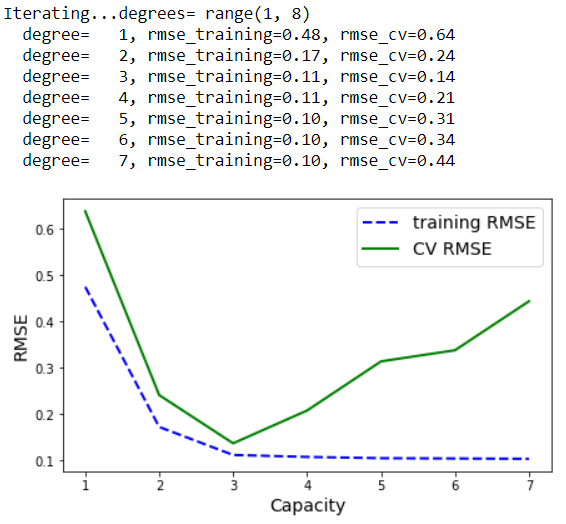
\includegraphics[width=0.9\textwidth]{sec5-gen-a}
    \caption{Capacity RMSE plot of training data and CV}
    \label{fig:gen_a}
\end{figure}

Figure \ref{fig:gen_a} shows that both the training RMSE and CV (generalization) RMSE decreses until the capacity (degree) is 3. The training erros are fairly high until then, which means that both the training and the generalization error are underfitting. After this point, the training RMSE keeps lowering, but the generalization error is increasing again. This means that the model is now overfitting! The point where the training RMSE and generalization error are close is at capacity = 3. This means that using a degree of 3 is the optimal choice. 
\\ \\
Figure \ref{fig:gen_a_alt} shows what happens if the degrees are increased even further.

\begin{figure}[H]
  \centering
    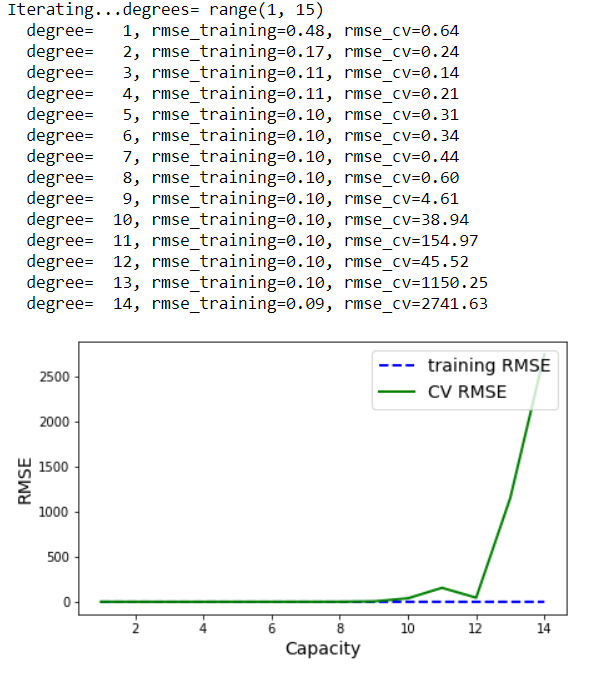
\includegraphics[width=0.9\textwidth]{sec5-gen-a-alt}
    \caption{Capacity RMSE plot of training data and CV with 14 degrees}
    \label{fig:gen_a_alt}
\end{figure}

It is not obvious to see on the plot, but looking at the numbers printed, it is seen that the capacity of 3 is again the most optimal. The RMSE will increase for CV after this point. The number of samples have not changed, so this ought to still be the case. Though, if the number of samples is increased, the optimal capacity is not one number. For example if the number of samples are increased to 300, both capacity 4 and 5 hold the lowest RMSE values for CV. This is obvious because the number of samples are higher and much closer to each other in value.

\end{document}